\ifx\PREAMBLE\UnDef
\documentclass{beamer}
\usepackage{tikz}
\usepackage[english]{babel}
% or whatever

\usepackage[latin1]{inputenc}
% or whatever
\usepackage{xifthen}
\usepackage{bsymb}

\newcommand{\always}{\mathop{\square}}
\newcommand{\eventually}{\mathop{\diamondsuit}}

\begin{document}
\else
\fi

\providecommand{\until}{\mathop{\mathcal{U}}}
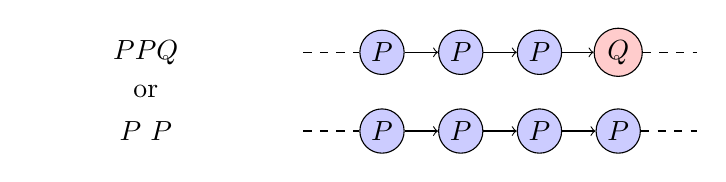
\begin{tikzpicture}[scale=0.5]
  \draw (-4,2) node[minimum width=3cm]{$P \limp P \until Q$};
  \draw (2,2) node(t1)[circle, draw, fill=blue!20!white, inner sep =
  2pt, minimum width=0.5cm]{$P$};
  \draw (4,2) node(t2)[circle, draw, fill=blue!20!white, inner sep =
  2pt, minimum width=0.5cm]{$P$};
  \draw (6,2) node(t3)[circle, draw, fill=blue!20!white, inner sep =
  2pt, minimum width=0.5cm]{$P$};
  \draw (8,2) node(t4)[circle, draw, fill=red!20!white, inner sep =
  2pt, minimum width=0.5cm]{$Q$};
  \draw[dashed] (0,2) -- (t1);
  \draw[->] (t1) -- (t2);
  \draw[->] (t2) -- (t3);
  \draw[->] (t3) -- (t4);
  \draw[dashed] (t4) -- (10,2);

  \draw (-4,1) node[minimum width=3cm]{or};
  \draw (-4,0) node[minimum width=3cm]{$P \limp \always P$};
  \draw (2,0) node(s1)[circle, draw, fill=blue!20!white, inner sep =
  2pt, minimum width=0.5cm]{$P$};
  \draw (4,0) node(s2)[circle, draw, fill=blue!20!white, inner sep =
  2pt, minimum width=0.5cm]{$P$};
  \draw (6,0) node(s3)[circle, draw, fill=blue!20!white, inner sep =
  2pt, minimum width=0.5cm]{$P$};
  \draw (8,0) node(s4)[circle, draw, fill=blue!20!white, inner sep =
  2pt, minimum width=0.5cm]{$P$};
  \draw[dashed] (0,0) -- (s1);
  \draw[->] (s1) -- (s2);
  \draw[->] (s2) -- (s3);
  \draw[->] (s3) -- (s4);
  \draw[dashed] (s4) -- (10,0);
  
\end{tikzpicture}

\ifx\PREAMBLE\UnDef
\end{document}
\else
\fi
